\chapter{Abstract Syntax}
\label{abschapter}

\section{Introduction}

Just as the quintessential step in object oriented design is
constructing a model of system concepts, constructing an abstract
syntax model is an essential first step in the design of a
modelling language. An abstract syntax model describes the
concepts in the language and their relationships to each other. In
addition, it also defines the rules that determine whether a model
written in the language is valid or not. These are the
well-formedness rules of the language.

Imagine a business modelling language suitable for modelling high
level business rules about business data. An appropriate language
for this domain might provide modelling concepts such as "data
model", "data entity", and "business rule". In addition, there
will be relationships between these concepts: a "data model" may
be composed of a number of "data entities". There will also be
rules describing the valid models that may be constructed in the
language, for instance, "a datamodel cannot contain data entities
with the same name" might be one such rule.

The concepts, relationships and rules identified during this step
will  provide a vocabulary and grammar for constructing models in
the language. This will act as a foundation upon which all other
artefacts of the language design process will be based.

This chapter describes the steps required to construct abstract
syntax models, along with examples of their application to the
definition of the abstract syntax model of a simple modelling
language.

\section{Modelling Abstract Syntax}

As stated, the purpose of an abstract syntax model is to describe
the concepts in a language and the relationships that exist
between those concepts. In the context of a language definition, a
concept is anything that represents a part of the vocabulary of
the language. The term abstract syntax emphasises a focus on the
the abstract representation of the concepts, as opposed to their
concrete representation. As a result, abstract syntax models focus
on the structural relationship that exist between language
concepts. Note that it is not the purpose of the abstract syntax
model to describe the semantics of the language. These aspects
will be described later.

An abstract syntax model should also describe  the rules by which
a model written in the language is deemed to be well-formed, i.e.
is syntactically valid. These provide a more detailed description
of the syntactical rules of the language than is possible by
describing the concepts and relationships alone. Well-formedness
rules are particularly useful when it comes to implementing a tool
to support the language as they can be used to validate the
correctness of models as they are created.

Constructing an abstract syntax model has much in common with
developing an abstract grammar for a programming language, with
the exception that the language is more expressive than that used
in programming language design.

Abstract syntax models are written in a metamodelling language. As
described in chapter \ref{xmfchapter}, the metamodelling language
we will use, called XMF, provides a number of modelling
abstractions suitable for modelling languages. For the purposes of
modelling abstract syntax only a subset of XMF will be required.
This is the subset suitable for capturing the static properties of
language concepts and well-formedness rules, and includes:

\begin{itemize}
\item Classes to describe the concepts in the language.
\item Packages to partition the model into manageable chunks where
necessary.
\item Attributes and associations to describe the relationships between
concepts.
\item Constraints, written in OCL, to express the well-formedness rules.
\item Operations, written in XOCL, to describe operations on the
state of a model.
\end{itemize}

\section{The Process}

There are a number of stages involved in the development of an
abstract syntax model: concept identification; concept modelling;
model architecting; model validation and model testing. These
stages are described below.

\subsection{Concept Identification}
\label{conceptidentification}

The first stage in modelling the abstract syntax of a language is
to utilise any information available to help in identifying the
concepts that the language uses, and any obvious rules regarding
valid and invalid models.

There are a number of useful techniques that can be used to help in
this process:

\begin{itemize}

\item Construct a list of candidate concepts in the language.
Focus on determining whether the concepts make sense as part of
the language's vocabulary. In particular, identify concepts
that match the following criteria:

\begin{itemize}
  \item Concepts that have names.
   \item Concepts that contain other concepts, e.g. a class containing attributes.
  \item Concepts that record information about relationships with other concepts, e.g. named associations between classes.
  \item Concepts that play the role of namespaces for named concepts.
  \item Concepts that exhibit a type/instance relationship.
  \item Concepts that are recursively decomposed.
  \item Concepts that are a part of an expression or are associated with expressions.
\end{itemize}

\item Build examples of models using the language.

\begin{itemize}
\item Utilise any notation that you think appropriate to represent
each type of concept. Use this notation to build models of meaningful/real world examples.
\item In the case of a pre-existing language there should be
resources already available to help in the identification of
concepts. These may include BNF definitions of the language
syntax, which can be translated into a metamodel and examples of
usage. Other sources of inspiration include existing tools, which
will provide automated support for building example models. Such
tools may also provide additional facilities for checking valid
and invalid models, which will be useful when identifying
well-formedness rules or may provide more detailed examples of the
language syntax.
\end{itemize}

\end{itemize}

Once some examples have been constructed, abstract away from them
to identify the generic language concepts and relationships between
concepts. It is often useful to annotate the examples with the
modelling concepts as a precursor to this step. Examples of invalid
models can also be used to help in the identification of
well-formedness rules.

It is important during this process to distinguish between the
concrete syntax of a language and its abstract syntax. Whilst it is
common for the structure of the abstract syntax to reflect its
concrete syntax, this need not be the case. For example, consider a
language which provides multiple, overlapping views of a small
number of core modelling concepts. In this case, the abstract
syntax should reflect the core modelling concepts, and not the
concrete syntax.

'Modelling the diagrams' is a common mistake made by many novice
modellers. If in doubt, ask the following questions when
identifying concepts:

\begin{itemize}
\item Does the concept have meaning, or is it there purely for
presentation? If the latter, then it should be viewed as concrete
syntax. An example might be a "Note", which clearly does not
deserve to be modelled as an abstract syntax concept.
\item Is the concept a derived concept or is it just a view
on a collection of more primitive concepts? If the latter, a
relationship should be defined between the richer concept and the
more primitive concept.
\end{itemize}

In general, the best abstract syntax models are the simplest ones.
Any complexity due to diagrammatical representation should be
deferred to the concrete syntax models.

\subsection{Use Cases}

A useful technique to aid in the identification of modelling
language concepts is to consider the different use cases
associated with using the language. This is almost akin to writing
an interface for a metamodel, i.e. a collection of operations that
would be used when interacting with the metamodel. Some typical
use cases might include creating and deleting model elements, but
may also include semantically rich operations such as transforming
or executing a model. The detailed descriptions that result from
the use case analysis can then be mined for modelling language
concepts.

\subsection{Concept Modelling}

Once concepts have been identified, standard object-oriented
modelling features, classes, packages, and associations are
applied to model the concepts in the language. There are many
examples of developing conceptual models available in the
literature, for instance \cite{larman} devotes a significant
amount of time to this subject.

In general, concepts will be described using classes, with
appropriate attributes used to capture the properties of the
concepts. Some concepts will have relationships to other concepts,
and these will be modelled as associations. Where it makes sense
to define categories of concepts, generalization can be used to
separate them into more general and more specific types of
concepts.

A useful strategy to apply at this stage is to reuse existing
language definitions where possible. There are a number of
techniques that can be used to achieve this, including:

\begin{itemize}
\item Extending or tailoring an existing metamodel to fit the
new language. This can be achieved by specializing classes from the
existing metamodel or by using package extension to import and
extend whole packages of concepts.
\item Utilising language patterns. A language pattern may be realised
as a framework of abstract classes that capture a repeatedly used
language structure, or by a package template (a parameterized package).
\end{itemize}

\noindent A full discussion of reuse techniques will be presented
in chapter \ref{langchapter}.

\subsection{Well-formedness Rules}

Once a basic model has been constructed, start identifying both
legal and illegal examples of models that may be written in the
language. Use this information to define a set of well-formedness
rules in OCL that rule out the illegal models. When defining
rules, look to identify the most general rules possible, and
investigate the implications of what happens when rules are
combined - sometimes rules can conflict in unexpected ways. There
are many books available that can help guide this process (see
\cite{oclBook} for example). Reusing existing language components
can also minimise the effort involved in writing well-formedness
rules, as constraints can be reused as well via inheritance.

\subsection{Operations and Queries}

Operations and queries should also be defined where appropriate.
Examples of operations include general utility operations such as
creating new model elements and setting attribute values, or
operations that act as test harnesses. Examples of queries might
include querying properties of models for use in constraints and
operations, or for validation purposes. Operations that change the
state of models should take any constraints into account, ensuring
that if a constraint holds before the operation is invoked, it
will continue to hold afterwards. Note that in general it is best
to focus on using operations to test out the model - avoid at this
point writing operations that implement other features of the
language such as semantics.

\subsection{Validation and Testing}

It is important to validate the correctness of the abstract syntax
model. Investing in this early on will pay dividends over full
language design lifecycle. A useful (static) technique for doing
this is to construct instances of the abstract syntax model that
match those of example models. An object diagram is a useful way
of capturing this information as it shows instances of classes
(objects) and associations (links). There are tools available that
will both help create object diagrams, and also check they are
valid with respect to a model and any OCL constraints that have
been defined.

The best means of testing the correctness of a language definition
is to build a tool that implements it. Only then can the language
be tested by end users in its entirety. The architecture of a tool
that facilitates the rapid generation of tools from metamodels
will be discussed in detail in later versions of this book.

\section{Case Study}

The best way to learn about metamodelling is to tackle a real
example. An example of a simple, but widely known modelling
language, is a StateMachine. StateMachines are widely used as a
notation for modelling the effect of state changes on an object.
StateMachines are a good starting point for illustrating
metamodelling as they are simple, but have enough features to
exercise many facets of the metamodelling process.

Many different types of State Machine languages are described in
the literature. This chapter will concentrate on a simplified form
of StateMachines. Later chapters will show this language can be
extended with richer modelling capabilities.

As shown in figure \ref{smexample}, a StateMachine is essentially a
visual representation of states and transitions. The StateMachines
described here are a form of object-oriented (OO) StateMachines. As
such, they describe the state changes that can occur to an instance
of a class, in this case a Library Copy.

\begin{figure}[htb]
\begin{center}
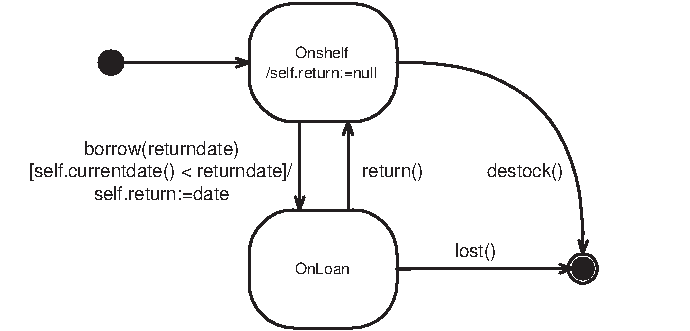
\includegraphics[width=11cm]{AbstractSyntax/figures/SMExample.pdf}
\caption{An example of a StateMachine} \label{smexample}
\end{center}
\end{figure}

StateMachines have an initial state and an optional final state,
which are represented by a filled circle and double filled circle
respectively. In addition, StateMachines provide guards, actions
and events. Guards are owned by transitions, and are boolean
expressions that must evaluate to true before a transition can be
invoked. Guards are represented by square brackets after an event
name. An example of a guard is shown in figure \ref{smexample}
attached to the borrow event.

In order to describe the effect of a transition on the state on an
object, actions can also be attached to transitions. Actions are
written in an action language, which in this case is XOCL. Actions
can also be attached to states, and are invoked when the state is
first entered. An example of an action that sets the returndate of
a Copy is shown in the figure \ref{smexample}.

Finally, events are associated with transitions via an event.
Events have a name and some optional parameters. It is the receipt
of an event that causes a transition to be triggered. Events can be
generated by StateMachine actions.

\subsection{Identification of Concepts}

Based on the example shown in figure \ref{smexample}, the
following candidate concepts can be immediately identified:

\begin{description}
\item [State]  A named representation of the state of an object at
a particular point in time.

\item [Initial State] The initial state that the object is
in when it is created.

\item [Final State] The final state of the object - typically when
the object has been destroyed.

\item [Transition] A state change. A transition has a source and target
state.

\item [Event] A named event that causes a transition to occur.

\item [Action] An executable expression that may be attached to
a transition or a state. Actions are invoked whenever the
transition occurs, or a state is entered.

\item [Guard] A boolean expression which must be evaluated to
be true before a transition can occur.

\end{description}

Figure \ref{stmannotated} shows the same StateMachine model 'marked
up' with some of the identified concepts.

\begin{figure}[htb]
\begin{center}
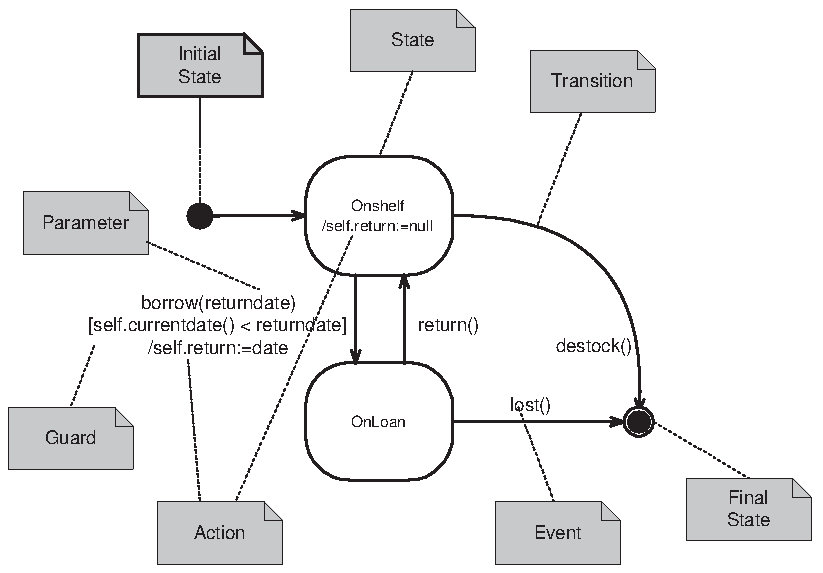
\includegraphics[width=13cm]{AbstractSyntax/figures/SMAnnotated.pdf}
\caption{An annotated example of a StateMachine}
\label{stmannotated}
\end{center}
\end{figure}

At this stage it would also be possible to start listing the
concepts that are used in the body of guards and actions, such as
equality ("="), assignment (":="). This would be a precursor to
constructing models of the expression language they belong to.
However, this is not necessary because we assume that the
expression languages are already defined (in this case OCL and
XOCL).

\subsection{The Model}

Once some candidate concepts have been identified, the next step
is to construct the model.

An important question to ask at this point is whether each concept
is a distinct abstract syntax concept. States and Transitions are
clearly core to StateMachines, as they capture the central concepts
of state and state change. However, initial states and final states
could be argued not to be concepts in their own right. An initial
state can be modelled as an attribute of the StateMachine, whilst a
final state can be viewed as a property of the instance (the
instance has been deleted).

The result of constructing the abstract syntax model is shown in
figure \ref{stmabs1}.

\begin{figure}[htb]
\begin{center}
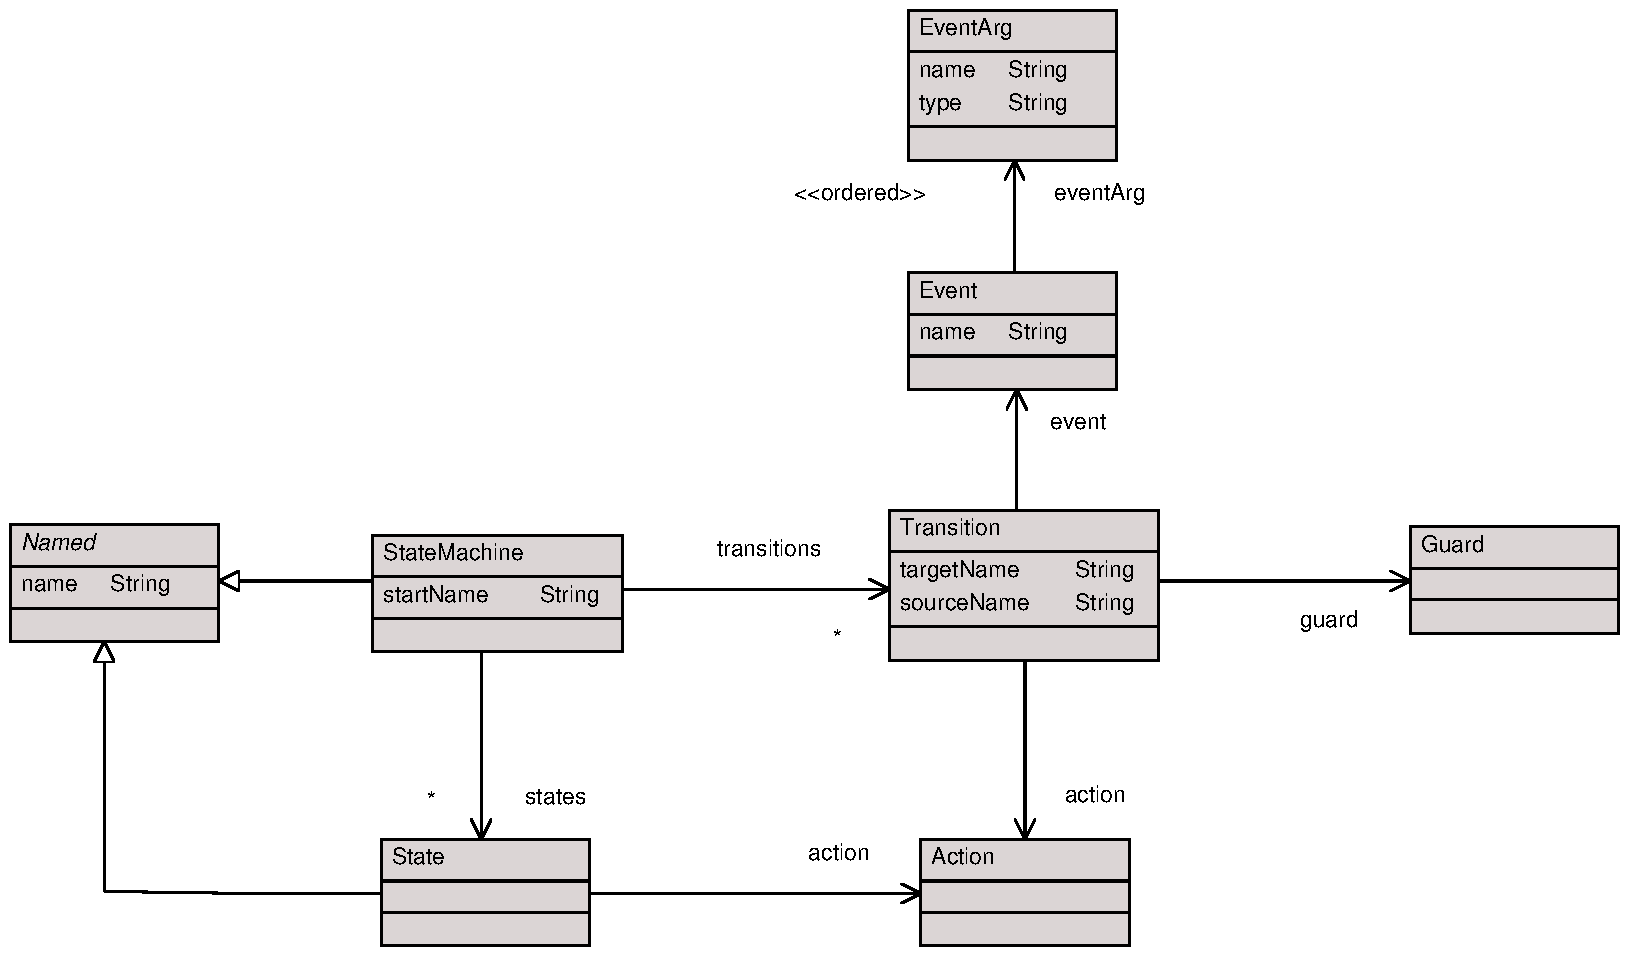
\includegraphics[width=16cm]{AbstractSyntax/figures/SMAbs1.pdf}
\caption{An abstract syntax metamodel for StateMachines}
\label{stmabs1}
\end{center}
\end{figure}

There are a number of points to note about the model:

\begin{itemize}
\item Transitions reference their source and target states by
name. \item The actions and guards of states and transitions are
associated with the classes Action and Guard respectively. These
will be extended in the next section to deal with the language
needed to construct action and guard expressions. \item The
initial state of a StateMachine is represented by the attribute
{\em startName}. This is a good example of where the abstract
syntax does not match the concrete syntax one to one (in other
words, the visual representation of an initial state does not have
a counterpart class concept in the abstract syntax model). \item
Transitions are optionally associated with an event, which has a
name, and a sequence of arguments, which have a name and a type.
\end{itemize}

\subsection{Metamodel Reuse}

Once the basic concepts have been identified, the next step is to
identify opportunities for reusing existing metamodelling
concepts. There are two main places where this occurs.

Firstly, elements may specialise existing metamodel concepts. As
described in chapter \ref{langextension}, XMF provides a framework
of classes that are specifically designed for reuse when
metamodelling. In this example, one type of element that can be
reused is a NamedElement. Rather than inventing a new concept, we
can specialise this class wherever we want a concept to have a
name.

Before proceeding we must be clear about the exact properties of
the concept we are specialising. A brief look at the XCore
framework in section \ref{framework} tells us that named elements
also have owners. Moreover, named elements also inherit the
ability to be navigated to via pathnames (this is defined in their
concrete syntax definition). While there are a number of classes
that have a name, it does not make sense for them all to have
owners and to be accessible via pathnames. In particular, concepts
like Event, Message and their arguments types do not have this
property. The classes State and StateMachine on the other hand,
do. A State has a name and it is likely that it will need to know
about the state machine it belongs to. A StateMachine will be
owned by a class.

Another concept that we may wish to specialise is a Contained
element. A contained element has an owner, but does not have a
name. In this example, Transition fits that criteria.

Reuse can also be achieved by referencing existing metamodel
concepts. For example, in order to precisely write guards and
actions, a metamodel of an appropriate expression language will be
required. It is much easier to reuse an existing metamodel that
provides the necessary expression types than to build this model
from scratch. In this case the XOCL metamodel provides a good
match: it includes both constraint style (OCL) expressions and
action style expressions.

Thus, the model needs to be changed so that actions and guards are
associated with XOCL expressions. A convenient way of achieving
this is to use the class XMF::Operation to encapsulate the
expression bodies. The resulting metamodel is shown in figure
\ref{stmabs2}

\begin{figure}[htb]
\begin{center}
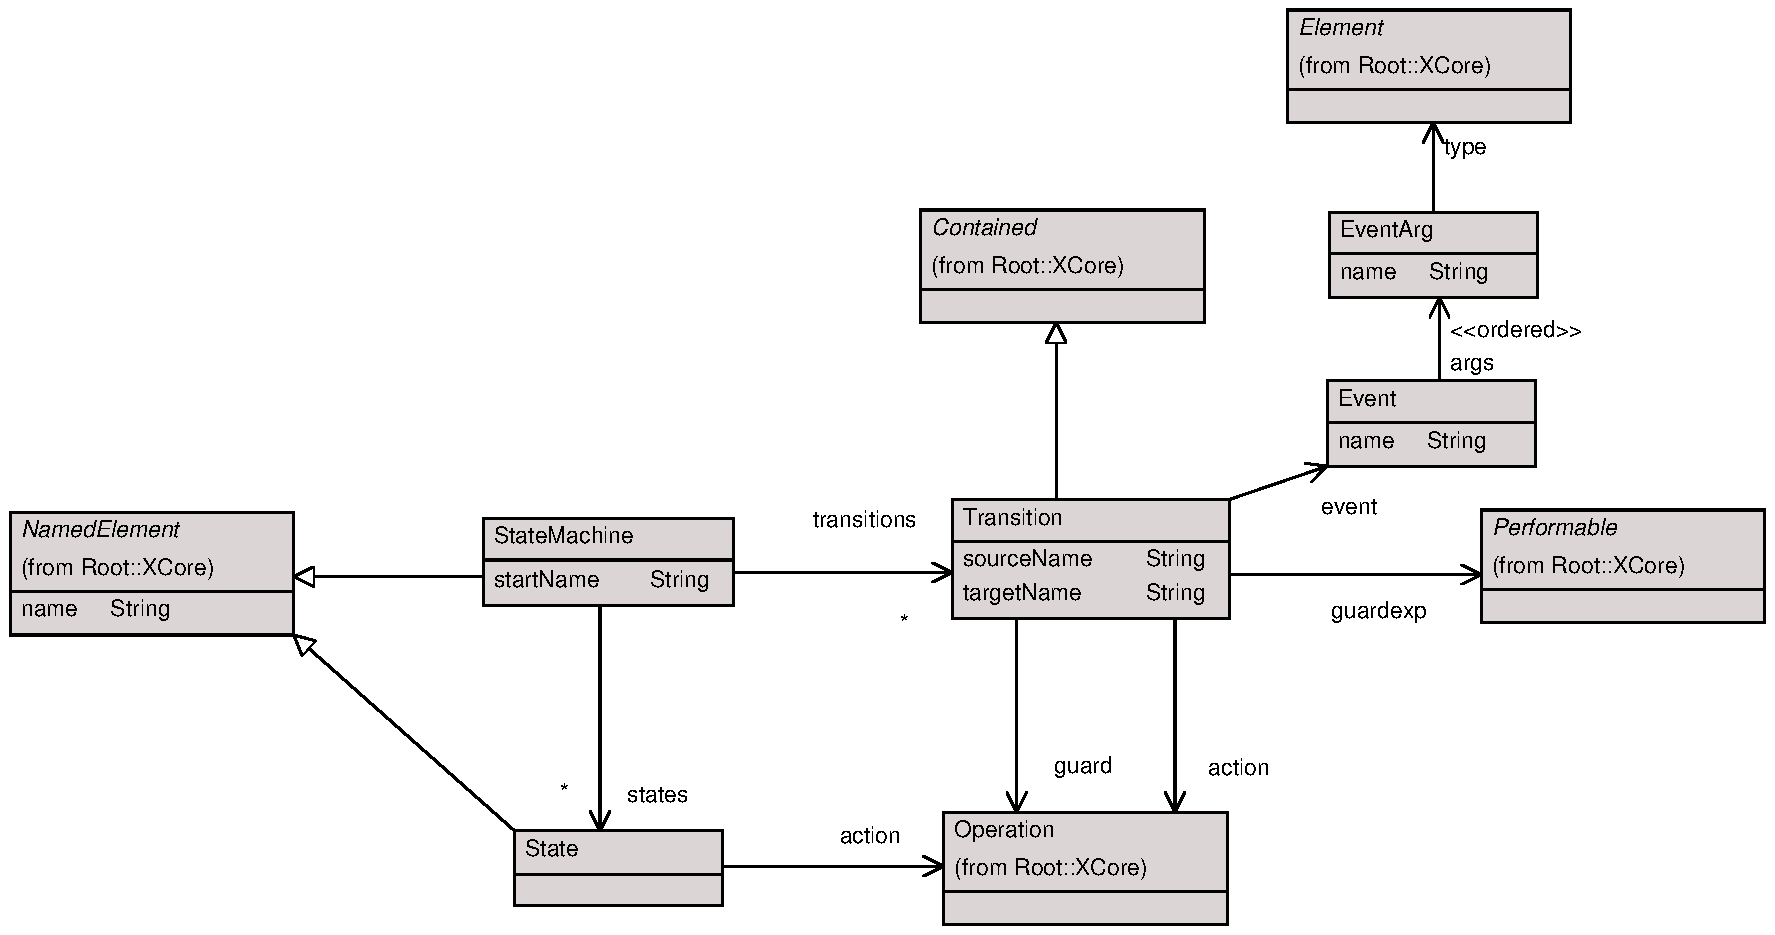
\includegraphics[width=16cm]{AbstractSyntax/figures/SMAbs2.pdf}
\caption{An extended abstract syntax metamodel for StateMachines}
\label{stmabs2}
\end{center}
\end{figure}

Finally, the type of a parameter is replaced with the class
XMF::Element. This enables parameter types to be of any XMF type,
thereby reusing XMF's type machinery.

\subsection{Well-formedness Rules}

Once the concepts and relationship in the StateMachine language
have been identified,  well-formedness rules can be defined. Here
are some examples:

\noindent Firstly, it must be the case that all states have a
unique names:

\begin{lstlisting}
context StateMachine
  @Constraint StatesHaveUniqueNames
    states->forAll(s1 |
      states->forAll(s2 |
        s1.name = s2.name implies s1 = s2))
  end
\end{lstlisting}\noindent Secondly, the initial state of the StateMachine must be
one the StateMachine's states:

\begin{lstlisting}
context StateMachine
  @Constraint StatesIncludeInitialState
    states->exists(s | s.name = startName)
  end
\end{lstlisting}\subsection{Operations}

Next, operations are added that will be used to create elements of
a StateMachine. The first adds a state to a StateMachine and sets
the owner of State to be the StateMachine. Note the operation
cannot be invoked if the name of the new State conflicts with an
existing state in the StateMachine, thus ensuring that
StatesHaveUniqueNames constraint is not broken.

\begin{lstlisting}
context StateMachine
  @Operation addState(state:StateMachines::State)
    if not self.states->exists(s | s.name = state.name) then
      self.states := states->including(state);
      self.state.owner := self
    else
      self.error("Cannot add a state that already exists")
  end
\end{lstlisting}\noindent The second adds a transition (again setting the owner to
be the StateMachine):


\begin{lstlisting}
context StateMachine
  @Operation addTransition(transition:StateMachines::Transition)
    self.transitions := transitions->including(transition);
    self.transition.owner := self
  end
\end{lstlisting}\noindent Similar operations will need to be defined for deleting
states and transitions.

The following query operations are defined. The first returns the
initial state of the StateMachine provided that it exists, or
returns an error. An error is a pre-defined operation on XMF
elements that is used to report errors.

\begin{lstlisting}
context StateMachine
  @Operation startingState()
    if states->exists(s | s.name = startName) then
       states->select(s | s.name = startName)->sel
    else
      self.error("Cannot find starting state: " + startName)
    end
  end
\end{lstlisting}\noindent The second returns the set of transitions starting from a
particular state:

\begin{lstlisting}
context StateMachine
  @Operation transitionsFrom(state:String)
     transitions->select(t | t.sourceName = state)
  end
\end{lstlisting}\subsection{Validating the StateMachine Metamodel}

In figure \ref{smsnapshot} a partial snapshot corresponding to the
StateMachine in figure \ref{smexample} is shown.

\begin{figure}[htb]
\begin{center}
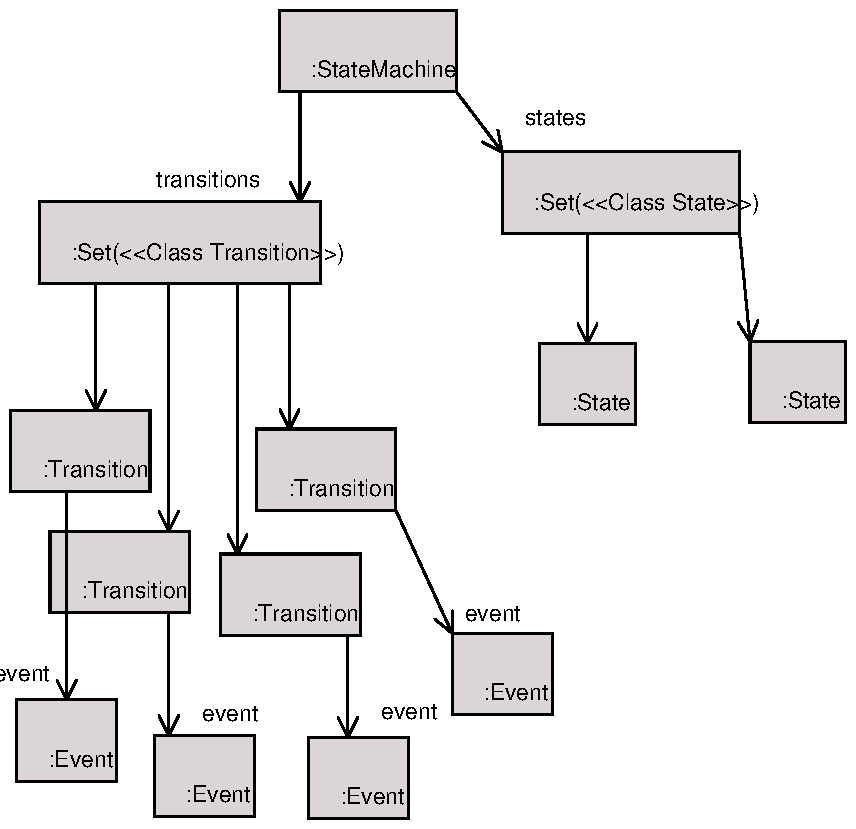
\includegraphics[width=11cm]{AbstractSyntax/figures/SMSnapshot.pdf}
\caption{A snapshot (object diagram) corresponding to figure
\ref{smexample}} \label{smsnapshot}
\end{center}
\end{figure}

A number of different properties of the model can be usefully
tested by snapshots. These include checking the well-formedness
rules and query operations by running them against the snapshot.

However, this is about as far as we can go. At this point, the
model is just a model of the abstract syntax and nothing more.
Other aspects of the StateMachine language, including its concrete
syntax and semantics, must be modelled before a precise, self
contained language definition is obtained. These aspects will be
explored in the following chapters.

\section{Conclusion}

This chapter has examined the process and modelling language
required to model the abstract syntax of languages. The result is
a definition of the concepts in a language and the relationship
and rules that govern them. However, this is just a first step
towards a complete definition of the language. Only once the
concrete syntax and semantics of the language are modelled does it
become a complete definition of the StateMachine language.
